\documentclass[headrule,footrule]{foils}


%%
%%%  Macros
%%%
%%% fonts-sil-charis for IPA in week 5

\newcommand{\logo}{HG2002 (2021)}
\usepackage[hidelinks]{hyperref}

\newcommand{\header}[3]{%
  \title{\vspace*{-2ex} \large 
    HG2002 Semantics and Pragmatics
% \thanks{Creative
%       Commons Attribution License: 
%       you are free to share and adapt as long as you give 
%       appropriate credit and add no additional restrictions: 
%       \protect\url{https://creativecommons.org/licenses/by/4.0/}.
%     }
    \\[2ex] \Large  \emp{#2} \\ \emp{#3}}
  \author{\blu{Francis Bond}   \\ 
    \normalsize  \textbf{Division of Linguistics and Multilingual Studies}\\
    \normalsize  \url{http://www3.ntu.edu.sg/home/fcbond/}\\
    \normalsize  \texttt{bond@ieee.org}}
  \MyLogo{\logo}
  % \MyLogo{奈良女子大学:欧米言語情報理論II}
  \date{#1
    \\  \url{https://bond-lab.github.io/Semantics-and-Pragmatics/}
\\[.5ex] \footnotesize Creative  Commons Attribution License:  you are free to share and adapt 
\\[-.25ex] \footnotesize   as long as you give    appropriate credit and add no
additional restrictions: 
\\ \small  \protect\url{https://creativecommons.org/licenses/by/4.0/}.
}
  % \renewcommand{\logo}{#2}
  % \special{! /pdfmark where
  %   {pop} {userdict /pdfmark /cleartomark load put} ifelse
  %   [ /Author (Francis Bond)
  %   /Title (#1: #2)
  %   /Subject (HG2002: Semantics and Pragmatics)
  %   /Keywords (Semantics, Pragmatics, Meaning)
  %   /DOCINFO pdfmark}
  %   }
  \hypersetup{%
    final       = true,
    colorlinks  = true,
    urlcolor    = blue,
    citecolor   = blue,
    linkcolor   = MidnightBlue,
    unicode     = true,
    pdfauthor   = {Francis Bond},
    pdfkeywords = {Semantics, Pragmatics, Meaning},
    pdftitle    = {#1: #2},
    pdfsubject  = {HG2002 Semantics and Pragmatics; License CC BY 4.0}
  }
}


\usepackage[a4paper,landscape]{geometry}
%\usepackage[dvips]{xcolor}
\usepackage[dvipsnames,x11names]{xcolor}
\usepackage{graphicx}
\newcommand{\blu}[1]{\textcolor{blue}{#1}}
\newcommand{\grn}[1]{\textcolor{green}{#1}}
\newcommand{\hide}[1]{\textcolor{white}{#1}}
\newcommand{\emp}[1]{\textcolor{red}{#1}}
\newcommand{\txx}[1]{\textbf{\textcolor{blue}{#1}}}
\newcommand{\lex}[1]{\textbf{\mtcitestyle{#1}}}


\usepackage{amsmath,latexsym}
\usepackage{pifont}
\renewcommand{\labelitemi}{\textcolor{violet}{\ding{227}}}
\renewcommand{\labelitemii}{\textcolor{purple}{\ding{226}}}

\newcommand{\subhead}[1]{\noindent\textbf{#1}\\[5mm]}

\newcommand{\Bad}{\emp{\raisebox{0.15ex}{\ensuremath{\mathbf{\otimes}}}}}
\newcommand{\bad}{*}

\newcommand{\com}[1]{\hfill \textnormal{(\emp{#1})}}%
\newcommand{\cxm}[1]{\hfill \textnormal{(\txx{#1})}}%
\newcommand{\cmm}[1]{\hfill \textnormal{(#1)}}%

\usepackage{relsize,xspace}
\newcommand{\into}{\ensuremath{\rightarrow}\xspace}
\newcommand{\ent}{\ensuremath{\Rightarrow}\xspace}
\newcommand{\nent}{\ensuremath{\not\Rightarrow}\xspace}
\newcommand{\tot}{\ensuremath{\leftrightarrow}\xspace}
\usepackage{url}
\newcommand{\lurl}[1]{\MyLogo{\url{#1}}}

\usepackage{mygb4e}
\let\eachwordone=\itshape
\newcommand{\lx}[1]{\textbf{\textit{#1}}}
\newcommand{\ix}{\ex\it}

\newcommand{\cen}[2]{\multicolumn{#1}{c}{#2}}
%\usepackage{times}
%\usepackage{nttfoilhead}
\newcommand{\myslide}[1]{\foilhead[-25mm]{\raisebox{12mm}[0mm]{\emp{#1}}}\MyLogo{\logo}}
\newcommand{\myslider}[1]{\rotatefoilhead[-25mm]{\raisebox{12mm}[0mm]{\emp{#1}}}}
%\newcommand{\myslider}[1]{\rotatefoilhead{\raisebox{-8mm}{\emp{#1}}}}

\newcommand{\section}[1]{\myslide{}{\begin{center}\Huge \emp{#1}\end{center}}}



\usepackage[lyons,j,e,k]{mtg2e}
\renewcommand{\mtcitestyle}[1]{\textcolor{teal}{\textsl{#1}}}
%\renewcommand{\mtcitestyle}[1]{\textsl{#1}}
\newcommand{\ja}[1]{\mtcitestyle{\makexeCJKactive #1\makexeCJKinactive}}
\newcommand{\chn}{\mtciteform}
\newcommand{\zsm}{\mtciteform}
%\newcommand{\cmn}[1]{make\cjkactive\mtciteform#1\makecjkinactive}
\newcommand{\iz}[1]{\textup{\texttt{\textcolor{blue}{\textbf{#1}}}}}
\newcommand{\con}[1]{\textsc{#1}}
\newcommand{\gm}{\textsc}
\newcommand{\cmp}[1]{{[\textsc{#1}]}}
\newcommand{\sr}[1]{\ensuremath{\langle}#1\ensuremath{\rangle}}
\usepackage[normalem]{ulem}
\newcommand{\ul}{\uline}
\newcommand{\ull}{\uuline}
\newcommand{\wl}{\uwave}
\newcommand{\vs}{\ensuremath{\Leftrightarrow}~}
%%% theta role
\newcommand{\tr}[1]{\textcolor{Chartreuse4}{\textsc{#1}}}
%%% theta grid
\newcommand{\grid}[1]{\ensuremath{\langle}\tr{#1}{\ensuremath{\rangle}}}

%%%
%%% Bibliography
%%%
\usepackage{natbib}
%\usepackage{url}
\usepackage{bibentry}
%\usepackage{CJKutf8}


\usepackage{fontenc}
\usepackage{polyglossia}
\setmainlanguage{english}
\setotherlanguages{tamil}
\setmainfont[Ligatures=TeX]{TeX Gyre Pagella}
\setsansfont[Ligatures=TeX]{TeX Gyre Heros}
\newfontfamily\ipafont{Charis SIL}
\newcommand\ipa[1]{\mtcitestyle{\ipafont #1}}


\usepackage{xeCJK}
\makexeCJKinactive
\newcommand{\zh}[1]{\mtcitestyle{\makexeCJKactive #1\makexeCJKinactive}}
%\newcommand{\ja}[1]{\makexeCJKactive #1\makexeCJKinactive}
\setCJKmainfont{Noto Sans CJK JP}
\setCJKsansfont{Noto Sans CJK SC}
\setCJKmonofont{Noto Sans CJK SC}

\newfontfamily\tamilfont[Script=Tamil]{Noto Sans Tamil}
\newfontfamily\tamilfontsf[Script=Tamil]{Noto Sans Tamil}
\newcommand{\tam}[1]{\texttamil{#1}}
%%% From Tim
\newcommand{\WMngram}[1][]{$n$-gram#1\xspace}
\newcommand{\infers}{$\rightarrow$\xspace}


\usepackage{rtrees,qtree}
\renewcommand{\lf}[1]{\br{#1}{}}
\usepackage{avm}
%\avmoptions{topleft,center}
\newcommand{\ft}[1]{\textsc{#1}}
\renewcommand{\val}[1]{\textit{#1}}
\newcommand{\typ}[1]{\textit{#1}}
\avmfont{\sc}
\avmvalfont{\sc}
\renewcommand{\avmtreefont}{\sc}
\avmsortfont{\it}


%%% From CSLI book
\newcommand{\mc}{\multicolumn}
\newcommand{\HD}{\textbf{H}\xspace}
\newcommand{\el}{\< \>}
\makeatother
\long\def\smalltree#1{\leavevmode{\def\\{\cr\noalign{\vskip12pt}}%
\def\mc##1##2{\multispan{##1}{\hfil##2\hfil}}%
\tabskip=1em%
\hbox{\vtop{\halign{&\hfil##\hfil\cr
#1\crcr}}}}}
\makeatletter

%\usepackage{tipa}
\usepackage{multicol}


\newcommand{\task}{\marginpar{\large ~~~\textbf{?}}}
\newcommand{\sh}[1]{\href{https://www.arthur-conan-doyle.com/index.php?title=#1}{#1}}

\usepackage{tikz}
\usepackage{tikz-qtree}
\usepackage{forest}



\begin{document}
\header{Lecture 7}{Context and Inference}{}\maketitle


\myslide{Overview}

\begin{itemize}\addtolength{\itemsep}{-1ex}
\item Revision: Participants
  \begin{itemize}
  \item Thematic Roles
  \item Classifiers and Noun Classes
  \end{itemize}
  \item Reference and Context
  \item Knowledge as Context
  \item Information Structure
  \item Inference
  \item Conversational Implicature
  \item Next Lecture: \emp{Chapter 8: Speech as Action}
\end{itemize}

%%%
%%% this changes each year, so keep separate
%%%
\include{schedule}


\section{Revision: Participants}


\myslide{Thematic Roles}
\begin{itemize}
\item  Thematic roles are parts of the sentence that 
correspond to the participants in the situation 
described
\item  They classify relations between entities in a situation

\item  Roles link different alternations
\begin{exe}
  \ex \eng{Kim patted Sandy}
  \ex \eng{Sandy was patted by Kim}
\end{exe}
\end{itemize}

\myslide{Thematic Roles}
\begin{itemize}
\item \txx{AGENT} (takes \eng{deliberately, on purpose, what did X do?})
  \begin{itemize}
  \item  Volitional, typically animate
  \item Typically \textsc{subject}
  \item  \eng{\ul{Kim} kicked Sandy}
  \end{itemize}
\item  \txx{PATIENT} (\eng{What happened to X?})
  \begin{itemize}
  \item  Undergoes change in state usually, both animate and 
    inanimate
  \item Typically \textsc{object}
  \item  \eng{Kim kicked \ul{Sandy}}
  \end{itemize}

\item  \txx{THEME}
  \begin{itemize}
  \item  Moved, location or state is described
  \item Typically \textsc{object}
  \item  \eng{He put \ul{the book} on the shelf}
  \end{itemize}
\newpage
\item  \txx{EXPERIENCER}
  \begin{itemize}
  \item   Non-volitional, displaying awareness of action, state
  \item Typically \textsc{subject}
  \item   \eng{\ul{He} heard thunder}
  \end{itemize}
\item  \txx{BENEFICIARY}
  \begin{itemize}
  \item   for whose benefit the action was performed
  \item   Typically indexed by "for" PP and "to" PP in English
  \item  \eng{They gave \ul{me} a present}
  \item  \eng{They gave a present \ul{to me}}
  \item  \eng{They made a present \ul{for me}}
  \end{itemize}
\newpage  
\item  \txx{LOCATION}
  \begin{itemize}
  \item  Place
  \item Typically indexed by locative PPs in English
  \item  \eng{I live \ul{in Jurong}}
  \end{itemize}

\item  \txx{GOAL}
  \begin{itemize}
  \item  towards which something moves (lit or metaphor)
 \item  Typically indexed by "to" PP in English 
 \item  \eng{She handed her form \ul{to him}}, \eng{She handed \ul{him} her form}
  \end{itemize}
\item  \txx{SOURCE}
 \begin{itemize}
 \item  from which something moves or originates
 \item  Typically indexed by "from" PP in English
 \item  \eng{We gleaned this \ul{from the Internet}}  
 \end{itemize}
\newpage
\item  \txx{INSTRUMENT/MANNER}
  \begin{itemize}
  \item  Means by which action is performed
  \item  Can be indexed by "with" PP in English
  \item  \eng{I ate breakfast \ul{with chopsticks}}
  \end{itemize}
\item  \txx{STIMULUS}
  \begin{itemize}
  \item  Usually used in connection with EXPERIENCER
  \item  \eng{\ul{The lightning} scared him}
\end{itemize}
\end{itemize}


\myslide{Theta-Grid}
\begin{itemize}\addtolength{\itemsep}{-0.9ex}
% \item  Goal: Explanation for the syntax-semantics 
% interface.
\item Verbs can be described with their \txx{valence}
  (\txx{theta-grid}, \txx{subcategorization})

 \begin{itemize}
 \item  \lex{give}: V $\langle$\ul{AGENT}, THEME, BENEFICIARY$\rangle$
 \item  underlined role maps to subject
 \item  order of roles allows prediction of grammatical function
 \end{itemize}
\item  This is used to link the meaning with the realization
\item Distinguish (with fuzzy boundaries) between
  \begin{itemize}
  \item \txx{participant roles}: depend on the verb --- in the grid (\txx{arguments})
    \\ obligatory; part of meaning; idiosyncratic syntax; 
 \\ participate in alternations 
  \item \txx{non-participant roles}: combine freely --- not in the grid (\txx{adjuncts})
    
  \end{itemize}
\item Theta Roles are semantic NOT syntactic
\end{itemize}

\myslide{Linking Grammatical Relations and Thematic Roles}
\begin{itemize}
\item    Thematic roles typically map onto grammatical 
  functions systematically
  \begin{itemize}
  \item  AGENT is usually the subject
  \item  PATIENT is usually the object
  \end{itemize}
\item  It is possible to predict how arguments are linked to 
  the verb from their thematic roles, and hence their 
  grammatical functions.
\item \txx{Thematic Hierarchy} The higher you are in the
  hierarchy the more likely to be subject (then object, then indirect,
  then argument PP, then adjunct PP
  \begin{small}
    \[ \mbox{AGENT} > \left\{\begin{array}[c]{l} \mbox{RECIPIENT} \\
        \mbox{BENEFICIARY} \end{array} \right\} >
    \left\{\begin{array}[c]{l} \mbox{THEME} \\
        \mbox{PATIENT} \end{array} \right\} > \mbox{INSTRUMENT} >
    \mbox{LOCATION} \]
  \end{small}
  \begin{itemize}
  \item  Generally true across languages
  \end{itemize}
\end{itemize}


\myslide{Dowty's Proto-Arguments}
\begin{itemize}
\item  The \txx{Agent} Proto-Role (Dowty 1991)
\begin{itemize}
\item  Volitional;  Sentient (and/or perceptive)
\item  Causes event or change of state;  Movement
\end{itemize}
\item  The \txx{Patient} Proto-Role
\begin{itemize}
\item  Change of state; Incremental theme (i.e. determines aspect)
\item  Causally affected by event
\item  Stationary (relative to movement of proto-agent).     
\end{itemize}
\item   when a verb takes a subject and an object
  \begin{itemize}
  \item  the argument with the greatest number of Proto-Agent 
    properties will be the one selected as \textsc{subject}
  \item  the one with the greatest no. of Proto-Patient properties 
    will be selected as \textsc{object}
  \end{itemize}
\end{itemize}

\myslide{Alternations}
\begin{itemize}
\item  Many verbs can have multiple theta-grids
  \begin{exe}
    \ex
    \begin{xlist}
      \ex \eng{Kim broke the window with the hammer}
      \ex \eng{The hammer broke the window}
      \ex \eng{The window broke}
    \end{xlist}
    \ex
    \begin{xlist}
      \ex \eng{I cut the cake with the knife}
      \ex \eng{This cake cuts easily}
    \end{xlist}
  \end{exe}  
\item  The relations between them are called \txx{alternations}
\item  English Verb Classes and Alternation (Levin 1993)
\end{itemize}



\myslide{Voice}
\MyLogo{These are also alternations for Levin}
\begin{itemize}
\item  Another way to change the number of arguments is 
\txx{voice}: passive, middle
\begin{exe}
  \ex Transitive Passive
  \begin{xlist}
    \ex \eng{Kim ate Sandy}
    \ex \eng{Sandy was eaten by Kim}
  \end{xlist}
  \ex Ditransitive Passive
  \begin{xlist}
    \ex \eng{A gave B C;   A gave C to B}
    \ex \eng{C was given to B by A;   B was given C by A}
  \end{xlist}
  \ex Transitive Middle (or just causative/inchoative)
  \begin{xlist}
    \ex \eng{They open the gate very quietly}
    \ex \eng{The gate opens very quietly}
  \end{xlist}
  \ex Intransitive Middle
  \begin{xlist}
    \ex \eng{The knife cuts the cake well}
    \ex \eng{The knife cuts well}
  \end{xlist}
\end{exe}
\end{itemize}



\myslide{Classifiers and Noun Classes}
\MyLogo{}
\begin{itemize}
\item  Many languages include special ways to classify 
nouns
\begin{itemize}
\item  Noun Classifiers (Bantu, Yidi , \ldots) 
\item  Numeral Classifiers (Chinese, Malay, Japanese, \ldots)
  \begin{itemize}
  \item English group nouns: \lex{flock, mob, group, pack, \ldots}
  \end{itemize}
\item  Gender (German, Spanish, \ldots)  
\end{itemize}
\item Classifiers can be marked on the noun, on the verb, on a
  separate word (a classifier) or on all words
\end{itemize}

\myslide{What gets Classified?}
\MyLogo{Allan (2001)}
\begin{itemize}
\item \txx{Taxonomic Class}: Human, Animal, Tree, Female
\item \txx{Function}: piercing, cutting, writing instrument, for eating/drinking
\item \txx{Shape}: long, flat, round (1D, 2D, 3D)
\item \txx{Consistency}: rigid, flexible
\item \txx{Size}: grab in fingers, hand, $<$ human, $>$ human
\item \txx{Location}: towns
\item \txx{Arrangement}: row, coil, heap
\item \txx{Quanta}: head, pack, flock
\end{itemize}

\myslide{Noun Classes vs Classifiers}
\MyLogo{\citet{Dixon:1986}}

\noindent\begin{tabular}{lll}
  & \textbf{Noun classes} & \textbf{Classifiers} \\
Size & Small Finite Set & Large Number (low hundreds) \\
Realization & Closed Grammatical System & Separate Morpheme \\
Marking & Also outside the noun word & Only in the noun phrase
\end{tabular}

\begin{itemize}
\item Gender (noun class in e.g., German)
  \begin{itemize}
  \item typically 3 (Masculine, Feminine, Neuter)
  \item marked as inflection
  \item marked on determiners, adjective and nouns
  \end{itemize}
\item Numeral Classifiers (in e.g., Japanese)
  \begin{itemize}
  \item typically 30-80 in common use, hundreds exist
  \item separate classifier phrase (numeral/interrogative+classifier)
  \item classifier phrase modifies noun
  \end{itemize}
\end{itemize}

\myslide{Summary}
\MyLogo{}
\begin{itemize}
\item  Semantics motivates syntax
  \begin{itemize}
  \item  But most generalizations fail to cover all examples
  \end{itemize}
\item Argument structure and thematic roles link predicates and their arguments
  \begin{itemize}
  \item \blu{Remember the basic roles and examples}
  \end{itemize}
%\item Grammar relations and thematic roles
\item Dowty's Argument Selection Principle
  \\ prototypical agents and patients are subjects and objects 
\item Problems with thematic roles
\item Noun Classes and Classifiers
\end{itemize}

\section{Context and Inference}
\myslide{Overview}

\begin{itemize}%\addtolength{\itemsep}{-1ex}
\item Reference and Context
\item Knowledge as Context
\item Information Structure
\item Inference
\item Conversational Implicature
\end{itemize}



\section{Reference and Context}
\MyLogo{}

\myslide{Context-dependence is everywhere}



\begin{itemize}%\addtolength{\itemsep}{-1.5ex}
%\item It isn't only deictic expressions that require context
\item For example, in a book shop
  \begin{exe}
    \ex \eng{Have you got the new \ul{Saeed}?} \textnormal{``book by $\sim$''}
  \end{exe}
\item In a snooker (pool)  game
  \begin{exe}
    \ex \eng{I have two \ul{reds} left} ``red balls''
  \end{exe}
\end{itemize}
\newpage
\MyLogo{\lex{suit}: \href{http://www.catb.org/jargon/html/S/suit.html}{a person who habitually wears suits, as distinct from a techie or hacker.  See pointy-haired, burble, management, \ldots}}

\begin{itemize}
\item \txx{metonymy}: substituting the name of an attribute or feature for the name of the thing itself
  \begin{exe}
    \ex \eng{\ul{The ham sandwich} is at table three} ``person who ordered $\sim$''
    \ex \eng{I spent all morning with \ul{the suits}} ``person who wears $\sim$''
  \end{exe}
  \item \txx{synecdoche}: substituting the name of a part for the name of a thing (or vice-versa)
    (a kind of metonymy)
  \begin{exe}
    \ex \eng{We need some more willing \ul{hands}} ``person with $\sim$''
    \ex \eng{\ul{Brazil} won the world cup} ``the team from $\sim$''
  \end{exe}
\end{itemize}

\section{Knowledge as Context}

\myslide{Generalize to all knowledge}
\begin{itemize}
\item Knowledge to interpret utterances can come from multiple sources
  \begin{enumerate}
  \item The physical context of the utterance
    \\ \txx{Deixis}
  \item What has already been said
    \\ \txx{Discourse}
  \item Background and common knowledge
    \\ \txx{World knowledge}
  \end{enumerate}
\end{itemize}

\myslide{Fragments}
\begin{itemize}
\item In a dialogue, we often only add new knowledge
  \begin{exe}
    \ex 
    \begin{xlist}
      \ex \eng{Who moved these chairs?}
      \ex \eng{Sandy (did) [move these chairs]}
  \end{xlist}
    \ex 
    \begin{xlist}
      \ex \eng{Where are you going?}
      \ex \eng{[I am going] (to) Tokyo}
  \end{xlist}
  \end{exe}
\item Normally English requires a complete sentence, 
\item[\ldots] but here a \txx{fragment} is OK
\end{itemize}

\myslide{Discourse Topic}
\MyLogo{\url{http://lessonstream.org/2011/04/30/washing-clothes/}}
\begin{itemize}
\item It is much easier to understand an utterance if you know what
  it is about \citep{Bransford:Johnson:1972}

\item Giving the same text different titles changes your interpretation

\item Giving a discourse topic aids in understanding and retention

\end{itemize}

\myslide{Background Knowledge}

What knowledge do we need to interpret the following?

\begin{exe}
  \ex 
  \begin{xlist}
    \ex \eng{I'm hungry}
    \ex \eng{I'll lend you some money}
  \end{xlist}
  \ex 
  \begin{xlist}
    \ex \eng{Shall we get some icecream?}
    \ex \eng{I'm on a diet}
  \end{xlist}
  \ex 
  \begin{xlist}
    \ex \eng{Shall we lunch next week?}
    \ex \eng{It's Ramadan}
  \end{xlist}
 \ex 
  \begin{xlist}
    \ex \eng{Kim chased the dog with a stick}
    \ex \eng{Kim chased the dog with a bone}
    \ex \eng{Kim chased the dog with a broom}
    \ex \eng{Kim chased the dog with a white tail}
    \ex \eng{Kim chased the dog with a wound}

  \end{xlist}

\end{exe}

%\myslide{Mutual Knowledge}

\myslide{Formalizing Knowledge for Computers}

\begin{itemize}
\item There is a lot of work on making knowledge available to
  computers so that they can interpret text
  \begin{itemize}
  \item Formal ontologies (knowledge-based)
    \begin{itemize}
    \item Scripts
    \item Wordnets
    \item CYC
    \end{itemize}
  \item Example-based (compare to existing examples)
    \\ collect many fragments of existing knowledge
  \end{itemize}
\end{itemize}


\myslide{Knowledge Yielding Ontologies  
 for Transition-based Orgs}
\MyLogo{I do this}
\begin{center}
  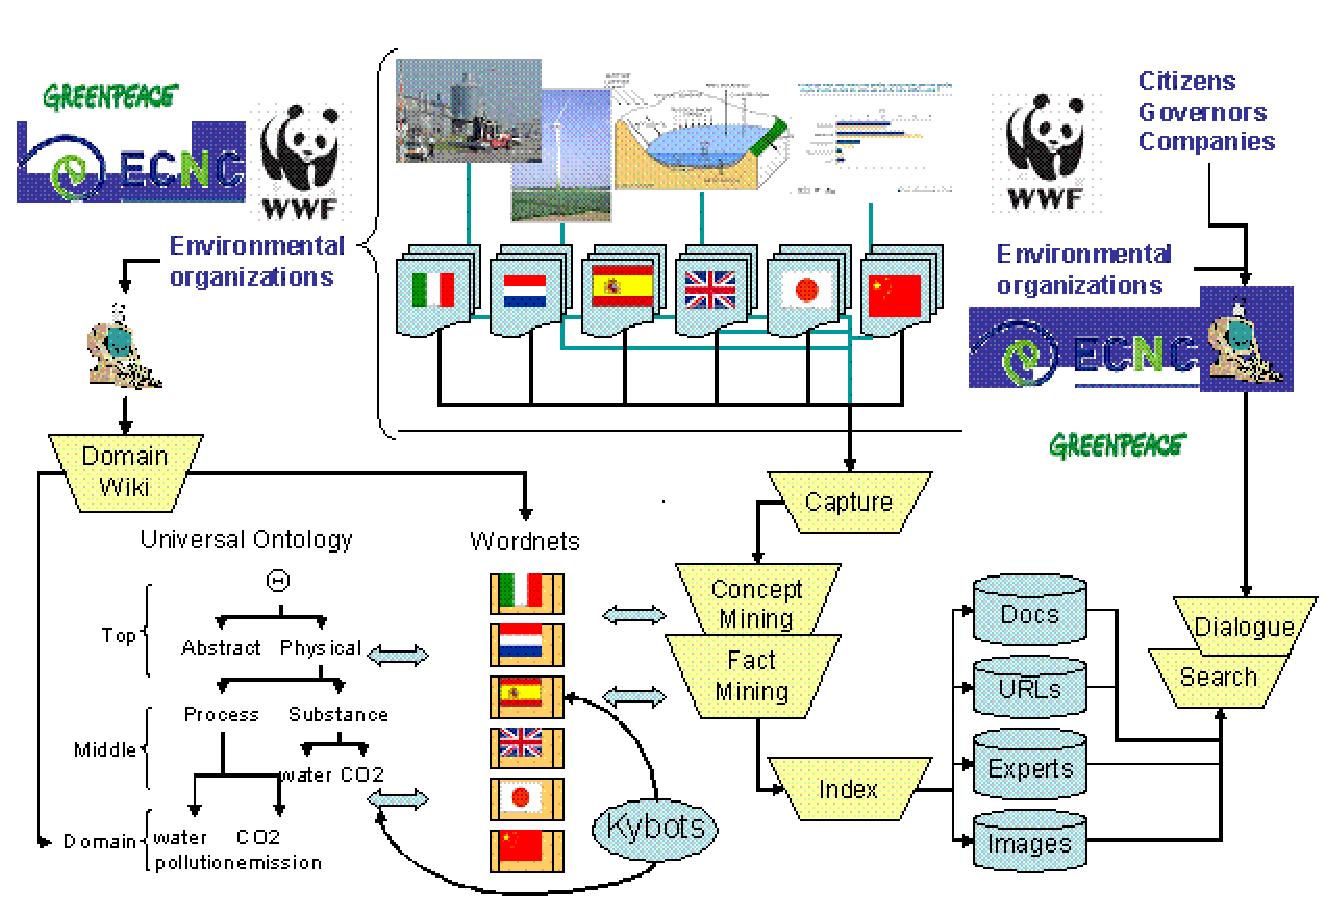
\includegraphics[width=0.8\textwidth]{pics/kyoto-project.eps}
\end{center}

\myslide{What can computers do?}
\MyLogo{}
\begin{itemize}
\item[Q] \eng{Do birds migrate through Turkey?}
\item[A] Yes.  \eng{The crane ($\subset$ bird) flies across Ankara ($\subset_{in}$ Turkey)}.
  \begin{quote}
    \large   fly$_1$ ($e_1$, crane$_5$($x_1$)),  across($e_2$,$e_1$,$x_2$), Ankara($x_2$).
  \end{quote}
  \begin{itemize}
  \item  \eng{through} and \eng{across} are both \textit{path} roles.
  \item \eng{fly} and \eng{migrate} are both \textit{motion} verbs.
  \item Ankara is in Turkey
  \end{itemize}
\item Why do this?
  \begin{itemize}
  \item Local environmental knowledge is often not translated into many languages
  \item Facts may only be recorded in a few documents
\end{itemize}
\end{itemize}


\section{Information Structure}

\myslide{Information status}
\begin{itemize}
\item Many languages signal whether information is \txx{new} or \txx{given}

\item We can signal this in many ways:
  \begin{exe}
      \ex \eng{I couldn't sleep last night}
      \ex
      \begin{xlist}
        \ex \eng{\ul{A dog next door} kept me awake}
        \ex \eng{\ul{This dog next door} kept me awake}
        \ex \eng{\ul{The dog next door} kept me awake}
        \ex \eng{\ul{That dog next door} kept me awake}
        \ex \eng{\ul{This} kept me awake}
        \ex \eng{\ul{It} kept me awake}
      \end{xlist}
  \end{exe}
\end{itemize}

\myslide{Givenness Hierarchy}
\MyLogo{\citet{Gundel:1993}}
\bigskip
\begin{small}
 \hspace*{-5em} \begin{tabular}{ccccccccccc}
 \textbf{Given} &&&&&&&&&& \textbf{New}\\[2ex]
    in  & $>$ & activated  & $>$ & familiar  & $>$ & identifiable  & $>$ & referential  & $>$ & type \\
   focus &&&&&&&&&&        identifiable \\
             & & \eng{that} \\
    \eng{it} & & \eng{this} && \eng{that N}&&\eng{the N}&&\eng{this N}&&\eng{a N} \\
             & & \eng{this N} \\
    \\
  \end{tabular}
\end{small}
\begin{itemize}
\item The more known and salient something is, the more it is
  \txx{given} information
\end{itemize}

\myslide{Focus}

\begin{itemize}
\item We can also mark information structure with intonation
  \begin{exe}
    \ex \eng{\textsc{Henry} cleaned the kitchen}
    \begin{xlist}
      \ex \textbf{Given}: someone cleaned the kitchen
      \ex \textbf{New}: it was Henry \hfill \txx{cleft}
    \end{xlist}
    \ex \eng{Henry cleaned \textsc{the kitchen}}
    \begin{xlist}
      \ex \textbf{Given}: Henry cleaned something
      \ex \textbf{New}: it was the kitchen
    \end{xlist}
    \ex \eng{Henry \textsc{cleaned} the kitchen}
    \begin{xlist}
      \ex \textbf{Given}: Henry did something to the kitchen
      \ex \textbf{New}: he cleaned it
    \end{xlist}
  \end{exe}
\item The prominent part is the \txx{focus}
\end{itemize}
  
\myslide{Topic}

\begin{itemize}
\item Some languages have a special \txx{[sentence] topic}
  \begin{exe} %\small
    \ex \gll \jpn{nihon-wa} \jpn{josei-wa} \jpn{heikin} \jpn{jumyou-ga} \jpn{nagai} \\
    japan-\textsc{top} women-\textsc{top} {average} {life expectancy}-\textsc{nom}
    long \\
    \trans As for Japan, as for women, the average life expectancy is long.
    \trans The average life expectancy of women in Japan is long.
    \ex \gll \jpn{N\`age}  \jpn{sh\`u} {} \jpn{y\`ezi} \jpn{d\`a} \\
    that tree {} leaves big \\
    \trans As for that tree, the leaves are big
    \trans That tree has big leaves. / That tree's leaves are big.
  \end{exe}
\item This differs a little from a subject 
  \\ (typically you can have none or multiple topics)
\end{itemize}

\section{Inference}

\myslide{Anaphoric Reference}
\MyLogo{In bridging, the referent is different, but linked in some way.}
\begin{itemize}
\item A pronoun (or definite nominal) can refer back to something
  earlier in the discourse
  \begin{exe}
    \ex 
    \begin{xlist}
    \ex \eng{I tripped over a dog. \ul{The dog} bit me.} \hfill \txx{definite}
    \ex \eng{I tripped over a dog. \ul{The beast} bit me.} \hfill \txx{definite}
    \ex \eng{I tripped over a dog. \ul{It} bit me.} \hfill \txx{pronominal}
    \ex \eng{I tripped over a dog. \ul{The tail} tangled me.} \hfill \txx{bridging}
    \ex \eng{I tripped over a dog. $\phi$ bit me.} \hfill \txx{zero}
  \end{xlist}
  \ex 
 \begin{xlist}
   \ex \eng{I left early.  I had a train to catch.}
   \trans \textnormal{Inference: I left early \textbf{because} I had a train to catch.}
 \end{xlist}
\end{exe}
\item People use inference to 
  \begin{itemize}
  \item Interpret pronouns and nominals
  \item More generally, to link information together
  \end{itemize}
\end{itemize}
 
\section{Conversational Implicature}


\myslide{Cooperation in Conversation}
\MyLogo{\citet{Grice:1975}}
\begin{itemize}
\item \txx{Cooperative Principle}: people cooperate in conversation
  \begin{quote}
    ``Make your conversational contribution such as is required, at the stage at which it occurs, by the accepted purpose or direction of the talk exchange in which you are engaged.''
  \end{quote}
\item \txx{Implicature}
  \begin{quote}
    The aspect of meaning that a speaker conveys, implies, or suggests
    without directly expressing.
  \end{quote}
  \begin{exe}
    \ex \eng{Did you do the reading?}
    \ex \eng{I meant to.}
    \trans \textnormal{Implicates: No}
  \end{exe}

\end{itemize}

\myslide{Gricean Maxims}
\MyLogo{\citet{Grice:1975}}
\begin{description}
\item [\txx{Maxim of Quantity}] ~
  \begin{itemize}
  \item Make your contribution as informative as is required (for the current purposes of the exchange).
  \item Do not make your contribution more informative than is required.
  \end{itemize}
\item [\txx{Maxim of Quality}] ~
  \begin{itemize}
  \item Do not say what you believe to be false.
  \item Do not say that for which you lack proper evidence.
  \end{itemize}
\newpage
\item [\txx{Maxim of Relation}] ~
  \begin{itemize}
  \item Be relevant.
  \end{itemize}
\item [\txx{Maxim of Manner}] ~
  \begin{itemize}
  \item Be perspicuous [= be easily understood]
  \item Avoid obscurity of expression.
  \item Avoid ambiguity
  \item Be brief (avoid unnecessary prolixity)
  \item Be orderly
  \end{itemize}
\end{description}

\myslide{An Example of implicature}

Speech that seems to violate the maxims will evoke \txx{implicatures}
(inferences about the reason why the speaker violated the maxim(s)).
This is because the hearer assumes the speaker is acting in accordance
with the Cooperative Principle, and is rational.
\begin{exe}
  \ex A: \eng{Can you tell me the time?}
  \trans Lit: Do you have the ability to tell me the time?
  \ex B: \eng{Well, the milkman has come.}
  \trans Lit.: The milkman came at some time prior to the time of speaking.
\end{exe}
\newpage
What is meant:
\begin{itemize}
\item [A] Do you have the ability to tell me the time of the present moment, as standardly indicated on a watch, and if so, please do so tell me what time it is.
\item [B] No, I don’t know the exact time of the present moment, but I can provide some information from which you may be able to deduce the approximate time, namely the milkman, who delivers milk at 6:30am,  came at some time prior to the time of speaking.
\end{itemize}

\begin{itemize}
\item [A] flouted Manner --- why not request that you are told the time?
\item [B] flouted Relation --- what does this have to do with the time?
\end{itemize}

\myslide{Generalized Conversational Implicatures}
\begin{itemize}
\item When no special knowledge is required in the context to calculate the additional conveyed meaning
  \begin{exe}
    \ex \eng{Did you bring the flowers and the card?}
    \ex \eng{I brought the card.}
    \trans \textnormal{Implicature: but not the flowers.}
  \end{exe}  
\end{itemize}


\myslide{Particularized Conversational Implicatures}

Most of our conversations take place in very specific contexts in
which locally recognized inferences are assumed.

\begin{exe}
  \ex \eng{Hey Terry, are you coming to the party tonight?}
  \ex \eng{My parents are visiting.}
\end{exe}

Note that all implicatures are \txx{defeasible}: they can be canceled
without a contradiction.

\begin{exe}
  \ex \eng{But I can still come.}
\end{exe}

\myslide{Scalar Implicatures}
\MyLogo{Extended into the Horn Scale: classic example is numbers}
\newcommand{\horn}[1]{\ensuremath{\langle}\,#1\,\ensuremath{\rangle}}
\newcommand{\set}[1]{\{#1\}}

Certain information is communicated by choosing a word which
expresses one value from a scale of values. 

\begin{exe}
  \ex	$\langle$ \eng{all, most, many, some, few} $\rangle$
  \ex	$\langle$ \eng{always, often, sometimes} $\rangle$
\end{exe}

We should choose the word from the scale which is the most informative
and truthful in the circumstances (Quantity and Quality):

\begin{exe}
  \ex \eng{I’m doing a major in Linguistics and I’ve completed some of the required subjects
  \ex \eng{They are often late.}
  \ex	I got some of these antiques in London – hang on, actually I think I got most of them 	there.} \hfill (defeasible)
\end{exe}
\myslide{Horn Scales}
\MyLogo{\url{http://www.personal.uni-jena.de/~mu65qev/wikolin/index.php?title=Horn_scale&redirect=no}}
 To form a
Horn scale \horn{$S,W$}, two words ($S$ and $W$) must satisfy the following
conditions:
\begin{enumerate}\addtolength{\itemsep}{-2ex}
\item[(i)] $A(S)$ must entail $A(W)$ for some arbitrary sentence frame $A$;
\item[(ii)] $S$ and $W$ must be equally lexicalized;
\item[(iii)] $S$ and $W$ must be about the same semantic relations, or
  from the same semantic field. 
\end{enumerate}
  \begin{itemize}
\item Words on the scale implicate the negation of words on their left
  \begin{itemize}
  \item \horn{\eng{always, often, sometimes}}.
  \item \horn{\eng{\ldots, 5, 4, 3, 2, 1}}.
  \item \horn{\eng{hot, warm, lukewarm, cold}}.
  \item \horn{\eng{the},  \set{\eng{a},\eng{some}}}.
  \end{itemize}
\end{itemize}



\myslide{Conventional Implicatures}
\MyLogo{}

Conventional implicatures are non-truth conditional inferences that
are not derived from superordinate pragmatic principles like the
[Gricean] maxims, but are simply attached by convention to particular
lexical items.

They are non-cancellable:
\begin{exe}
  \ex
  \begin{xlist}
    \ex \eng{She was poor, but honest.}
    \ex \eng{*She was poor but honest, and was in fact rich.}
  \end{xlist}
\end{exe}

\myslide{Flouting the maxims}
\begin{itemize}
\item Quantity:	(In answer to \eng{Tell me about him!}:) 
  \eng{He has a nice personality.}
\item Quality:	(In response to something stupid someone did:) 
  \eng{That was brilliant!}
\item Relation:	(In response to \eng{Can I go out and play?}:) 
\eng{Did you finish your homework?}
\item Quality:
  \begin{exe}
    \ex \eng{My car breaks down every five minutes} \hfill hyperbole
    \ex \eng{I’ve got millions of bottles of wine in my cellar} \hfill figure of speech
    \ex \eng{Queen Victoria was made of iron} \hfill a metaphor
    \ex \eng{I love it when you sing out of tune} \hfill irony or sarcasm
  \end{exe}
\end{itemize}
%% FIXME add some manner flouting

\myslide{What happens when we flout?}
\begin{itemize}
\item If someone doesn’t understand this, (e.g. someone from another
  culture), then what was originally intended to be a metaphor may
  result in a \txx{lie}.
\item We may flout: 
  \begin{itemize}
\item Quantity: 
  \begin{itemize}
  \item say  more than we need to indicate a sense of occasion, or respect
  \item  say less than we need, in order to be blunt, or rude
  \end{itemize}
\item Relation  
  \begin{itemize}
  \item to signal embarrassment
  \item to change the subject
  \end{itemize}
\item Manner
  \begin{itemize}
  \item for the   sake of humour
  \item to obscure information (parents talking in front of children)
  \item to show in-group status,  \ldots
  \end{itemize}
\end{itemize}
\end{itemize}


\myslide{Hedges}

When we \txx{flout}  a maxim, we can use \txx{hedges}:

\begin{exe}
\ex Quantity:
    \begin{exe}
    \ex \eng{\ul{As you probably know},} \ldots
    \ex \eng{\ul{To cut a long story short},} \ldots
  \end{exe}
\ex Quality:
  \begin{exe}
    \ex \eng{\ul{I’m not sure}, but I think they got divorced last year.}
    \ex \eng{\ul{As far as I’m aware}, Kim is still on medication.}
  \end{exe}
\ex Relation:
    \begin{exe}
    \ex \eng{\ul{I don’t know if this is will affect the bottom line}, but some of the numbers are  missing.}
  \end{exe}
  % b. This may seem beside the point, but we can’t ignore the impact of lower interest
  %  rates on these investments.
  %       c. Not that I’m changing the topic, but is this related to the budget?

\ex Manner:
 \begin{exe}
    \ex \eng{\ul{I'm not sure if this makes sense}, but the car had no lights.}
  \end{exe}
\end{exe}

% c. I don't know if this is clear at all, but I think the other car was reversing



% \myslide{Hedges and Conversational Implicatures}
% \begin{itemize}
% \item Hedges: show we know we are flouting a maxim
% \item \txx{Generalised conversational implicatures}
% \\ the inferences we make by assuming cooperation
% \item \txx{Particularised conversational implicatures}
% \\ local inferences  for a given situation
% \item \txx{Scalar implicatures} (Horn Scales)
% \\ one item on  a scale implicates all weaker items (and no stronger ones)
% \item \txx{Conventional implicatures}
% \\ implicatures attached to lexical items
% \end{itemize}



\myslide{Acknowledgments and References}
\MyLogo{}

\begin{itemize}\addtolength{\itemsep}{1ex}
\item Definitions from WordNet: \url{http://wordnet.princeton.edu/}

\item Some slides use material from Alexander Coupe

  
 \end{itemize}

\myslide{Truly Unique Things}

\begin{itemize} %\addtolength{\itemsep}{-1ex}
\item the music of Beethoven
\item the intuition of a woman
\item the obstinacy of an ass
\item the crowing of a cock
\item the song of a tit
\item the waywardness of the wind
\end{itemize}
\begin{flushright}
  Alas Smith and Jones (1986)
\end{flushright}
Mistakenly attributed to Oscar Wilde (1854 – 1900), who actually said:
\begin{quote}
``Intuition: the strange instinct that tells a woman she is right, whether she is or not.''  
\end{quote}



 % \item Images from
%   \begin{itemize}
%   \item the Open Clip Art Library: \url{http://openclipart.org/}
%   \item Steven Bird, Ewan Klein, and Edward Loper (2009) 
%      \textit{Natural Language Processing with Python}, O'Reilly Media
%     \\ \url{www.nltk.org/book}
% \end{itemize}
% \item Problems  partially based on exercises from Saeed (2003)
% \end{itemize}

%\myslide{Bibliography}
% Reading: Jurafsky and Martin (2008) Chapter 20
\small
\bibliographystyle{aclnat}
\bibliography{abb,mtg,nlp,ling}



\end{document}



%%% Local Variables: 
%%% coding: utf-8
%%% mode: latex
%%% TeX-PDF-mode: t
%%% TeX-engine: xetex
%%% End:

